\documentclass[11pt,letterpaper]{article}
\usepackage[utf8]{inputenc}
\usepackage[left=1in,right=1in,top=1in,bottom=1in]{geometry}
\usepackage{amsfonts,amsmath}
\usepackage{graphicx,float}
% -----------------------------------
\usepackage{hyperref}
\hypersetup{%
  colorlinks=true,
  linkcolor=blue,
  citecolor=blue,
  urlcolor=blue,
  linkbordercolor={0 0 1}
}
% -----------------------------------
\usepackage{fancyhdr}
\newcommand\course{Numerical Analysis}
\newcommand\hwnumber{5}                  % <-- homework number
\newcommand\NetIDa{Ryan Sh\`iji\'e D\`u} 
\newcommand\NetIDb{October 14th, 2022}
\pagestyle{fancyplain}
\headheight 35pt
\lhead{\NetIDa\\\NetIDb}
\chead{\textbf{\Large Worksheet \hwnumber}}
\rhead{\course}
\lfoot{}
\cfoot{}
\rfoot{\small\thepage}
\headsep 1.5em
% -----------------------------------
\usepackage{titlesec}
\renewcommand\thesubsection{(\arabic{section}.\alph{subsection})}
\titleformat{\subsection}[runin]
        {\normalfont\bfseries}
        {\thesubsection}% the label and number
        {0.5em}% space between label/number and subsection title
        {}% formatting commands applied just to subsection title
        []% punctuation or other commands following subsection title
% -----------------------------------
\setlength{\parindent}{0.0in}
\setlength{\parskip}{0.1in}
% -----------------------------------
\newcommand{\de}{\mathrm{d}}
\newcommand{\DD}{\mathrm{D}}
\newcommand{\pe}{\partial}
\newcommand{\mcal}{\mathcal}
%\newcommand{\pdx}{\left|\frac{\partial}{\partial_x}\right|}

\newcommand{\dsp}{\displaystyle}

\newcommand{\norm}[1]{\left\Vert #1 \right\Vert}
%\newcommand{\mean}[1]{\left\langle #1 \right\rangle}
\newcommand{\mean}[1]{\overline{#1}}
\newcommand{\inner}[2]{\left\langle #1,#2\right\rangle}

\newcommand{\ve}[1]{\boldsymbol{#1}}

\newcommand{\thus}{\Rightarrow \quad }
\newcommand{\fff}{\iff\quad}
\newcommand{\qdt}[1]{\quad \mbox{#1} \quad}

\renewcommand{\Re}{\mathrm{Re}}
\renewcommand{\Im}{\mathrm{Im}}
\newcommand{\E}{\mathbb{E}}
\newcommand{\lap} {\nabla^2}
\renewcommand{\div}{\nabla\cdot}

\newcommand{\csch}{\text{csch}}
\newcommand{\sech}{\text{sech}}


\newcommand{\hot}{\text{h.o.t.}}

\newcommand{\ssp}{\left.\qquad\right.}

\newcommand{\var}{\text{var}}
\newcommand{\cov}{\text{cov}}

%%%%%%%%%%%%%%%%%%%%%%%%%%%%%%%%%%%%%%%%%%%%%%%%%%
\makeatletter
\newcommand*{\mint}[1]{%
  % #1: overlay symbol
  \mint@l{#1}{}%
}
\newcommand*{\mint@l}[2]{%
  % #1: overlay symbol
  % #2: limits
  \@ifnextchar\limits{%
    \mint@l{#1}%
  }{%
    \@ifnextchar\nolimits{%
      \mint@l{#1}%
    }{%
      \@ifnextchar\displaylimits{%
        \mint@l{#1}%
      }{%
        \mint@s{#2}{#1}%
      }%
    }%
  }%
}
\newcommand*{\mint@s}[2]{%
  % #1: limits
  % #2: overlay symbol
  \@ifnextchar_{%
    \mint@sub{#1}{#2}%
  }{%
    \@ifnextchar^{%
      \mint@sup{#1}{#2}%
    }{%
      \mint@{#1}{#2}{}{}%
    }%
  }%
}
\def\mint@sub#1#2_#3{%
  \@ifnextchar^{%
    \mint@sub@sup{#1}{#2}{#3}%
  }{%
    \mint@{#1}{#2}{#3}{}%
  }%
}
\def\mint@sup#1#2^#3{%
  \@ifnextchar_{%
    \mint@sup@sub{#1}{#2}{#3}%
  }{%
    \mint@{#1}{#2}{}{#3}%
  }%
}
\def\mint@sub@sup#1#2#3^#4{%
  \mint@{#1}{#2}{#3}{#4}%
}
\def\mint@sup@sub#1#2#3_#4{%
  \mint@{#1}{#2}{#4}{#3}%
}
\newcommand*{\mint@}[4]{%
  % #1: \limits, \nolimits, \displaylimits
  % #2: overlay symbol: -, =, ...
  % #3: subscript
  % #4: superscript
  \mathop{}%
  \mkern-\thinmuskip
  \mathchoice{%
    \mint@@{#1}{#2}{#3}{#4}%
        \displaystyle\textstyle\scriptstyle
  }{%
    \mint@@{#1}{#2}{#3}{#4}%
        \textstyle\scriptstyle\scriptstyle
  }{%
    \mint@@{#1}{#2}{#3}{#4}%
        \scriptstyle\scriptscriptstyle\scriptscriptstyle
  }{%
    \mint@@{#1}{#2}{#3}{#4}%
        \scriptscriptstyle\scriptscriptstyle\scriptscriptstyle
  }%
  \mkern-\thinmuskip
  \int#1%
  \ifx\\#3\\\else_{#3}\fi
  \ifx\\#4\\\else^{#4}\fi  
}
\newcommand*{\mint@@}[7]{%
  % #1: limits
  % #2: overlay symbol
  % #3: subscript
  % #4: superscript
  % #5: math style
  % #6: math style for overlay symbol
  % #7: math style for subscript/superscript
  \begingroup
    \sbox0{$#5\int\m@th$}%
    \sbox2{$#5\int_{}\m@th$}%
    \dimen2=\wd0 %
    % => \dimen2 = width of \int
    \let\mint@limits=#1\relax
    \ifx\mint@limits\relax
      \sbox4{$#5\int_{\kern1sp}^{\kern1sp}\m@th$}%
      \ifdim\wd4>\wd2 %
        \let\mint@limits=\nolimits
      \else
        \let\mint@limits=\limits
      \fi
    \fi
    \ifx\mint@limits\displaylimits
      \ifx#5\displaystyle
        \let\mint@limits=\limits
      \fi
    \fi
    \ifx\mint@limits\limits
      \sbox0{$#7#3\m@th$}%
      \sbox2{$#7#4\m@th$}%
      \ifdim\wd0>\dimen2 %
        \dimen2=\wd0 %
      \fi
      \ifdim\wd2>\dimen2 %
        \dimen2=\wd2 %
      \fi
    \fi
    \rlap{%
      $#5%
        \vcenter{%
          \hbox to\dimen2{%
            \hss
            $#6{#2}\m@th$%
            \hss
          }%
        }%
      $%
    }%
  \endgroup
}

\begin{document}

\section{Conditional numbers based on different norms}
\subsection{}
Let $A \in \mathbb{R}^{n\times n}$ be defined by
\begin{equation*}
    A = %
    \begin{bmatrix}
      1      & 0      & 0      & 0      &  0      \\ 
      1      & 1      & 0      & 0      &  0      \\
      1      & 0      & 1      & 0      &  0      \\
      \vdots & \vdots & \vdots & \ddots &  \vdots \\
      1      & 0      & 0      & 0      &  1
    \end{bmatrix}.
\end{equation*}
Calculate $\kappa_1(A)$ and $\kappa_\infty(A)$. We see that a matrix can be well or ill-conditioned depending on the choice of norms.

\subsection{}
Indeed, we solve $A\ve x = \ve b$ and $A(\ve x+\Delta \ve x) = (\ve b+\Delta \ve b)$ where
\begin{align*}
    \ve b = \begin{bmatrix}
    1\\1\\\vdots\\1
    \end{bmatrix},\qquad \ve x = \begin{bmatrix}
    1\\0\\\vdots\\0
    \end{bmatrix},\qdt{and} \Delta\ve b = \begin{bmatrix}
    \epsilon\\0\\\vdots\\0
    \end{bmatrix}
\end{align*}
Check that we have for both norms:
\begin{align*}
    \frac{\norm{\Delta\ve x}}{\norm{\ve x}} \leq \kappa(A)\frac{\norm{\Delta\ve b}}{\norm{\ve b}}.
\end{align*}


\section{Conditional numbers and pivoted LU}
\subsection{}
Solve the matrix equation $A\boldsymbol x = \boldsymbol b$ with 
\begin{align*}
  A:=
  \begin{bmatrix}
    1       & 0  \\
    10^{4}  & 1
  \end{bmatrix}
  \qdt{ and }
  \boldsymbol b = \begin{bmatrix}
  0\\1
  \end{bmatrix}.
\end{align*}
What is $\kappa_\infty(A)$?

Consider a small perturbation $\Delta \boldsymbol b=[10^{-3},0]^\top$ being added to the right hand side, and solve again. Repeat with $\Delta \boldsymbol b =[0,10^{-3}]^\top$. You should see that small perturbations can, but do not have to have a large effect even for badly conditioned systems.

\subsection{}
Verify the following LU decomposition of a matrix $A$ without pivoting:
  $$
  A := \begin{bmatrix} 10^{-4} & 1\\ 1 & 1
  \end{bmatrix} = LU =
  \begin{bmatrix} 1 & 0\\ 10^4 & 1
  \end{bmatrix}
  \begin{bmatrix} 10^{-4} & 1\\ 0 & 1-10^4
  \end{bmatrix}
  $$ 
We have seen in the previous problem that solving a system with the matrix $L$ is sensitive to errors, i.e., it is poorly conditioned. However, the original $A$ matrix is well-conditioned.

Now the LU factorization of $A$ with pivoting is
\begin{align*}
PA = \begin{bmatrix} 1 & 1 \\ 10^{-4} & 1
  \end{bmatrix} = LU =
  \begin{bmatrix} 1 & 0\\ 10^{-4} & 1
  \end{bmatrix}
  \begin{bmatrix} 1 & 1\\ 0 & 1-10^{-4}
  \end{bmatrix}
\end{align*}
We see that the LU factors with pivoting are better conditioned.

\section{Conditional Number for Solving Linear System}  
\subsection{}
Find $\|{A}\|_2$ for the matrix 
\[
A = \begin{bmatrix} 1 & \varepsilon \\ \varepsilon & 1 \end{bmatrix},
\]where $\varepsilon \in (0,1)$ (Hint: for symmetric matrices $A$, the
eigenvalues of $A^T A$ are simply the squares of the eigenvalues of
$A$).

\subsection{}
Continued from previous item: Suppose that you have two systems
\begin{align*}
\begin{matrix}
x_1 + \varepsilon x_2 = b_1 \\
 \varepsilon x_1 + x_2 = b_2  
\end{matrix}\qquad \text{and}\qquad
\begin{matrix}
\tilde x_1 + \varepsilon \tilde x_2 = \tilde b_1 \\
 \varepsilon \tilde x_1 + \tilde x_2 = \tilde b_2
\end{matrix}
\end{align*}
where $\tilde{\boldsymbol b} = (\tilde b_1, \tilde b_2)^T$ is
approximately equal to ${\boldsymbol b}=( b_1, b_2)^T$, with a $5\%$
relative error, that is $\frac{\|{\tilde {\boldsymbol b} -
    {\boldsymbol b}}\|_2}{\|{{\boldsymbol b}}\|_2} \leq 0.05$.  Find
an upper bound for the relative error $\frac{\|\tilde {\boldsymbol x}
  - {\boldsymbol x}\|_2}{\|{\boldsymbol x}\|_2}$ where $\tilde
{\boldsymbol x} = (\tilde x_1, \tilde x_2)^T$ and ${\boldsymbol x} =
(x_1,x_2)^T$. This upper bound will depend on $\varepsilon$.

\section{Two forms of QR}
\subsection{}
We have two forms of QR:
\begin{figure}[H]
    \centering
    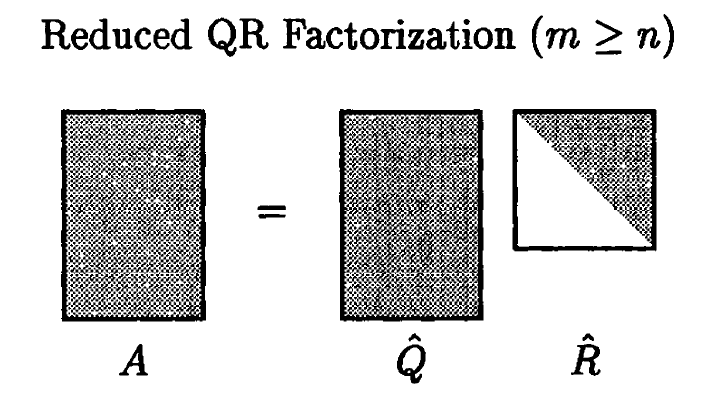
\includegraphics[width = 0.45\textwidth]{figs/TB_reducedQR}
    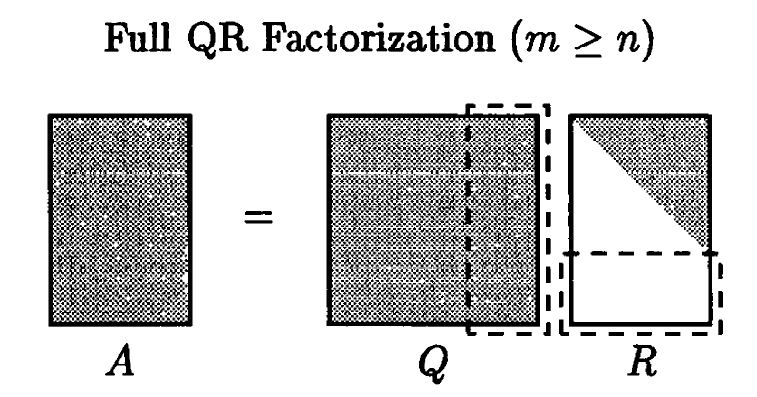
\includegraphics[width = 0.45\textwidth]{figs/TB_fullQR}
\end{figure}

\subsection{}
We can interpret the formula for the solution of the least-squared problem
\begin{align*}
    \hat R \ve x = \hat Q^\top \ve b
\end{align*}
by using the full form of QR.

\newpage
\section{Least squares and infections disease}
Let us assume an infectious disease with the following reported new
infections $I_i$ on each day $t_i$, for $i=1,\ldots,10$.
\begin{table}[h]\centering
  \caption{Number of new infections $I_i$ on days $t_i$.}
  \begin{tabular}{c||c|c|c|c|c|c|c|c|c|c|}
\hline
$t_i$: & 1 & 2 & 3 & 4 & 5 & 6 & 7 & 8 & 9 & 10\\ \hline
$I_i$: & 14 & 20 & 21 & 24 & 15 & 45 & 67 & 150 & 422 & 987\\ \hline
\end{tabular}
\end{table}
Using least squares fitting, we would like to understand the nature of
this growth. We consider two models to describe the connection between
time (i.e., days) $t$ and the number of new infections, both with 3
unknown parameters $(a,b,c)$:
\begin{equation*}%\label{poly}
  I(t) = a + b t + c t^2 \qquad \text{(polynomial model)}
\end{equation*}
\begin{equation*}%\label{exp}
  I(t) = a + bt + c\exp(t) \qquad \text{(exponential model)}
\end{equation*}
Our goal is to figure out which model describes the progression of the
infections better, and we use least squares fitting to figure that
out. Note that if a model would fit the data perfectly, $I(t_i) = I_i$
for all $i$. In general, you will not be able to find parameters that
satisfy this, and thus have to use least squares fitting (sometimes
this is also called \emph{regression}).

\subsection{} Formulate, assuming the polynomial model, the least squares
  problem for the parameters $\boldsymbol x=[a,b,c]^T$ by specifying the
  matrices $A$ and the vector $\boldsymbol b$:
  $$ \min_{\boldsymbol x\in \mathbb R^3}\|A\boldsymbol x - \boldsymbol
  b \|_2^2
  $$

\subsection{}  Same as above, but for the exponential model.

\subsection{} Use a QR-factorization in MATLAB or Python to solve these
  problems and plot the data as points, as well as the model as a
  line. Repeat using the normal equations $A^TA\boldsymbol x =
  A^T\boldsymbol b$.
\subsection{} To decide which model describes the data better, we need to
  compute the distance between the model and the data points. Take a
  look at the proof from class for how  the QR  factorization can be
  used to solve least squares  problems. In  particular, we found
  that:
  $$
  \|A\boldsymbol x  - \boldsymbol  b\|_2^2 \ge \|\boldsymbol b_2\|_2^2,
  $$ where $\boldsymbol b_2 = \hat{\hat Q}^\top\boldsymbol b$. We also
  found that this inequality is an equality if $\boldsymbol x$ solves
  the least squares problem. Thus, the norm or $\boldsymbol b_2$ is a
  measure of how well the model fits the data. Use this to decide
  which of the two models above describes the data better.

% \section{Conditional Number for the Hilbert Matrix}  
% The Hilbert matrix $H\in \mathbb R^{n\times n}$ is a matrix with
%   entries
%   $$
%   h_{ij} = \frac{1}{i+j-1}.
%   $$ Using MATLAB or Python, compute the 2-norm based condition
%   numbers for $n=3,5,10,20,25$.  Let's consider a relative right hand
%   side perturbation $\delta\boldsymbol b$ of a linear system with
%   $\|\delta\boldsymbol b\|_2/\|\boldsymbol b\|_2\approx
%   10^{-15}$. Write down the corresponding bounds $\|\delta\boldsymbol
%   x\|_2/\|\boldsymbol x\|_2$ from the theory we discussed in class.

%   Now, let's compute the actual error. Use the right hand side vector
%   with entries $b_i = \sum_{j=1}^n(j/(i+j-1))$ chosen such that the
%   solution vector has entries $x_i=i$. Now, Compute the numerical
%   solutions\footnote{Note that all these computations contain tiny
%     errors due to the final precision of computer computations.}
%   $\boldsymbol x$, then re-compute $\boldsymbol b=H\boldsymbol x$ and
%   compare the relative right hand side error and the relative error
%   in the solutions. How much are these better than the estimates you
%   got from the condition number?



\end{document}